\documentclass[11pt]{article}
\usepackage{amsmath, amsthm, amssymb,lscape, natbib}
\usepackage{mathtools}
\usepackage{subfigure}
\usepackage[font=footnotesize,labelfont=bf]{caption}
\usepackage{graphicx}
\usepackage{colortbl}
\usepackage{hhline}
\usepackage{multirow}
\usepackage{multicol}
\usepackage{setspace}
\usepackage[final]{pdfpages}
\usepackage[left=2.5cm,top=2.5cm,right=2.5cm, bottom=2.5cm]{geometry}
\usepackage{natbib} 
\usepackage{bibentry} 
\newcommand{\bibverse}[1]{\begin{verse} \bibentry{#1} \end{verse}}
\newcommand{\vs}{\vspace{.3in}}
\renewcommand{\ni}{\noindent}
\usepackage{xr-hyper}
\usepackage[]{hyperref}
\usepackage[capposition=top]{floatrow}
\usepackage{amssymb}
\usepackage{relsize}
\usepackage[dvipsnames]{xcolor}
\usepackage{fancyhdr}
\usepackage{tikz}
 
\pagestyle{fancy} % customize header and footer
\fancyhf{} % clear initial header and footer
%\rhead{Overleaf}
\lhead{\centering \rightmark} % this adds subsection number and name
\lfoot{\centering \rightmark} 
\rfoot{\thepage} % put page number (the centering command puts it in the middle, don't matter if you put it in right or left footer)

\def \myFigPath {../figures/} 
% BE CAREFUL WITH FIGNAMES, IN LATEX THEY'RE NOT CASE SENSITIVE!!
\def \myTablePath {../tables/} 

%\definecolor{mygreen}{RGB}{0, 100, 0}
\definecolor{mygreen}{RGB}{0, 128, 0}

\definecolor{citec}{rgb}{0,0,.5}
\definecolor{linkc}{rgb}{0,0,.6}
\definecolor{bcolor}{rgb}{1,1,1}
\hypersetup{
%hidelinks = true
  colorlinks = true,
  urlcolor=linkc,
  linkcolor=linkc,
  citecolor = citec,
  filecolor = linkc,
  pdfauthor={Laura G\'ati},
}


\geometry{left=.83in,right=.89in,top=1in,
bottom=1in}
\linespread{1.5}
\renewcommand{\[}{\begin{equation}}
\renewcommand{\]}{\end{equation}}

% New Options
\newtheorem{prop}{Proposition}
\newtheorem{definition}{Definition}[section]
\newtheorem*{remark}{Remark}
\newtheorem{lemma}{Lemma}
\newtheorem{corollary}{Corollary}
\newtheorem{conjecture}{Conjecture}

%\newtheorem{theorem}{Theorem}[section] % the third argument specifies that their number will be adopted to the section
%\newtheorem{corollary}{Corollary}[theorem]
%\newtheorem{lemma}[theorem]{Lemma}
%\declaretheorem{proposition}
%\linespread{1.3}
%\raggedbottom
%\font\reali=msbm10 at 12pt

% New Commands
\newcommand{\real}{\hbox{\reali R}}
\newcommand{\realp}{\hbox{\reali R}_{\scriptscriptstyle +}}
\newcommand{\realpp}{\hbox{\reali R}_{\scriptscriptstyle ++}}
\newcommand{\R}{\mathbb{R}}
\DeclareMathOperator{\E}{\mathbb{E}}
\DeclareMathOperator{\argmin}{arg\,min}
\newcommand\w{3.0in}
\newcommand\wnum{3.0}
\def\myFigWidth{5.3in}
\def\mySmallerFigWidth{2.1in}
\def\myEvenBiggerFigScale{0.8}
\def\myPointSixFigScale{0.6}
\def\myBiggerFigScale{0.4}
\def\myFigScale{0.3}
\def\mySmallFigScale{0.22}
\def\mySmallerFigScale{0.18}
\def\myTinyFigScale{0.16}
\def\myPointFourteenFigScale{0.14}
\def\myTinierFigScale{0.12}
\newcommand\numberthis{\addtocounter{equation}{1}\tag{\theequation}} % this defines a command to make align only number this line
\newcommand{\code}[1]{\texttt{#1}} %code %

\renewcommand*\contentsname{Overview}
\setcounter{tocdepth}{2}

% define a command to make a huge question mark (it works in math mode)
\newcommand{\bigqm}[1][1]{\text{\larger[#1]{\textbf{?}}}}

\begin{document}

\linespread{1.0}

\title{Materials 6 - More on IRFs}
\author{Laura G\'ati} 
\date{\today}
\maketitle

%%%%%%%%%%%%%%%%%%%%             DOCUMENT           %%%%%%%%%%%%%%%%%% 

\tableofcontents

%\listoffigures

%\newpage


\newpage
\section{Model summary, adding $\rho i_{t-1}$}
\begin{align}
x_t &=  -\sigma i_t +\hat{\E}_t \sum_{T=t}^{\infty} \beta^{T-t }\big( (1-\beta)x_{T+1} - \sigma(\beta i_{T+1} - \pi_{T+1}) +\sigma r_T^n \big)  \label{prestons18}  \\
\pi_t &= \kappa x_t +\hat{\E}_t \sum_{T=t}^{\infty} (\alpha\beta)^{T-t }\big( \kappa \alpha \beta x_{T+1} + (1-\alpha)\beta \pi_{T+1} + u_T\big) \label{prestons19}  \\
i_t &= \psi_{\pi}\pi_t + \psi_{x} x_t  + \textcolor{blue}{\rho i_{t-1}} + \bar{i}_t \label{TR}
\end{align}
\begin{equation}
\hat{\E}_t z_{t+h} =  \begin{bmatrix}\bar{\pi}_{t-1} \\ 0 \\ 0 \end{bmatrix}+ b\textcolor{blue}{hx}^{h-1}s_t  \quad \forall h\geq 1 \quad \quad b = gx \; hx \quad \quad \text{PLM} \label{PLM}
\end{equation}
\begin{equation}
\bar{\pi}_{t} = \bar{\pi}_{t-1} +k_t^{-1}\underbrace{\big(\pi_{t} -(\bar{\pi}_{t-1}+b_1s_{t-1}) \big)}_{\text{fcst error using (\ref{PLM})} } \quad \quad  \text{($b_1$ is the first row of $b$)}
\end{equation}
 \begin{align*}
k_t & = \mathbb{I}\times(k_{t-1}+1) + (1-\mathbb{I}) \times \bar{g}^{-1}  \label{gain} \numberthis\\
\mathbb{I} & = \begin{cases} 1 \quad \text{if} \; \theta_t \leq \bar{\theta}  \\ 0 \quad \text{otherwise.}\numberthis
\end{cases} \\
\theta_t & = |\hat{\E}_{t-1}\pi_t - \E_{t-1}\pi_t| / \sigma_s \quad \quad \text{CEMP criterion for the gain}\label{criterion}\numberthis
\end{align*}

The alternative criterion for the choice of gain is a recursive variant of the CUSUM-test (Brown, Durbin, Evans 1975):
\begin{enumerate}
\item Let $FE_t$ denote the short-run forecast error, and $\omega_t$ firms' estimate of the FE variance.
\item Let $\kappa \in (0,1)$ and $\tilde{\theta}$ be the new threshold value for the criterion.
\item Then for initial $(\omega_0, \theta_0)$, firms in every period estimate the criterion and the FEV as:
\begin{align}
 \omega_t & =  \omega_{t-1} + \kappa k_{t-1}^{-1}(FE_t^2 -\omega_{t-1})\\
\theta_t & =  \theta_{t-1} + \kappa k_{t-1}^{-1}(FE_t^2/\omega_t -\theta_{t-1})\\
k_t & = \mathbb{I}\times(k_{t-1}+1) + (1-\mathbb{I}) \times \bar{g}^{-1} \\
\mathbb{I} & = 1 \quad \text{if} \quad  \theta_t \leq \tilde{\theta}
\end{align}
\end{enumerate}

\newpage
\section{Compact notation - with lagged interest rate term in TR}
 \begin{align}
z_t & = A_p^{RE} \E_t z_{t+1} + A_s^{RE} s_t \label{LOM_RE} \\
z_t & = A_a^{LH} f_a(t) + A_b^{LH} f_b(t) + A_s^{LH} s_t \label{LOM_LH} \\
s_t & = P s_{t-1} + \epsilon_t \quad \quad \textcolor{blue}{\rightarrow} \quad s'_t  = hx \; s'_{t-1} + \epsilon'_t \label{exog} \\
 \quad \text{where} \quad 
 s'_t & \equiv \begin{pmatrix} r_t^n \\ \bar{i}_t \\ u_t \\ \textcolor{blue}{i_{t-1}}
 \end{pmatrix} \quad 
 hx  \equiv \begin{pmatrix} \rho_r & 0 & 0 & \textcolor{blue}{0} \\ 0& \rho_i & 0 & \textcolor{blue}{0} \\ 0&0& \rho_u & \textcolor{blue}{0}  \\ 
 \textcolor{blue}{gx_{3,1}}&\textcolor{blue}{gx_{3,2}}& \textcolor{blue}{gx_{3,3}} & \textcolor{blue}{gx_{3,4}}
 \end{pmatrix}  \quad 
 \epsilon'_t \equiv \begin{pmatrix}\varepsilon_t^{r} \\ \varepsilon_t^{i}  \\ \varepsilon_t^{u} \\ \textcolor{blue}{0} 
 \end{pmatrix}  \quad  \text{and } \quad \Sigma'  =  \begin{pmatrix} \sigma_r & 0 & 0 & \textcolor{blue}{0} \\ 0& \sigma_i & 0 & \textcolor{blue}{0}  \\ 0&0& \sigma_u & \textcolor{blue}{0}  \\ \textcolor{blue}{0}  & \textcolor{blue}{0} & \textcolor{blue}{0} & \textcolor{blue}{0} &
 \end{pmatrix} 
\end{align}

$i_{t-1}$ is an endogenous state and breaks the link that previously had $P = hx$; now this is no longer true. In particular, using Matlabby notation, $P = hx(1:3,1:3)$. What I don't get though is why $gx_{3,4} \neq \rho$? $\textcolor{mygreen}{\bigqm[5]}$ 

Adding $i_{t-1}$ to the state vector fortunately doesn't change $A^{RE}_p, A^{LH}_a$ or $A^{LH}_b$, but it does change $A^{RE}_s$ and $A^{LH}_s$. The latter two get an additional column to account for the new state variable. Also $f_a$ and $f_b$ need to be adjusted (replace $P$ by $hx$). With $g_{i, j} \; i=\pi,x, \; j=a,b$ unchanged from Materials 4, the new coefficient matrices are given by (new elements highlighted in \textcolor{blue}{blue}):
\begin{align}
A_s^{RE} &= \begin{pmatrix}   \frac{\kappa\sigma}{w}  &-\frac{\kappa\sigma}{w}  & 1-\frac{\kappa\sigma\psi_{\pi}}{w} & \textcolor{blue}{0}\\
 \frac{ \sigma}{w} &  -\frac{\sigma}{w} & -\frac{\sigma\psi_{\pi}}{w} & \textcolor{blue}{0}\\ 
 \psi_x( \frac{\sigma}{w}) + \psi_{\pi}( \frac{\kappa\sigma}{w}) & \psi_x(- \frac{\sigma}{w}) + \psi_{\pi}(- \frac{\kappa\sigma}{w}) +1 &  \psi_x(-\frac{\sigma\psi_{\pi}}{w}) + \psi_{\pi}( 1-\frac{\kappa\sigma\psi_{\pi}}{w}) & \textcolor{blue}{\rho}\end{pmatrix}  
\\
 A_s^{LH} & = \begin{pmatrix} g_{\pi s} \\ g_{x s} \\ \psi_{\pi}g_{\pi s} + \psi_xg_{x s} + \begin{bmatrix} 0 & 1& 0 & \textcolor{blue}{\rho}\end{bmatrix}
\end{pmatrix} \\
g_{\pi s} & = (1-\frac{\kappa\sigma\psi_{\pi}}{w} )\begin{bmatrix} 0&0&1 & \textcolor{blue}{0}\end{bmatrix} (I_{\textcolor{blue}{4}} - \alpha\beta \textcolor{blue}{hx})^{-1} -\frac{\kappa\sigma}{w}\begin{bmatrix} -1&1&0 & \textcolor{blue}{\rho} \end{bmatrix} (I_{\textcolor{blue}{4}} -\beta \textcolor{blue}{hx})^{-1}\\
g_{x s} & =  \frac{-\sigma\psi_{\pi}}{w} \begin{bmatrix} 0&0&1& \textcolor{blue}{0} \end{bmatrix}(I_{\textcolor{blue}{4}} - \alpha\beta \textcolor{blue}{hx})^{-1}  -\frac{\sigma}{w}\begin{bmatrix} -1&1&0 & \textcolor{blue}{\rho}\end{bmatrix}(I_{\textcolor{blue}{4}} -\beta \textcolor{blue}{hx})^{-1}
\end{align}

%%%%%%%%%%%  IRFs
\newpage
\section{Small deviations in $\pi$, large ones in $x$, overshooting - IRFs}

\subsection{Baseline figures, $\psi_x = 0, \psi_{\pi} = 1.5, \rho = 0$}
\begin{figure}[h!]
\subfigure[The observables for the specific shock sequence]{\includegraphics[scale = \mySmallFigScale]{\myFigPath materials6_observables_intrate_smoothing_rho0}} 
\subfigure[Inverse gain and drift for the specific shock sequence, CEMP and CUSUM criterion]{\includegraphics[scale = \mySmallFigScale]{\myFigPath materials6_gain_drift_cusum_intrate_smoothing_rho0} }
\caption{A baseline shock sequence,$\psi_x = 0, \psi_{\pi} = 1.5, \rho = 0$}
\end{figure}		
						


\newpage
\vspace{-0.5cm}
\subsection{IRFs when changing $\rho$}
\vspace{-0.5cm}
\begin{figure}[h!]
\subfigure[\colorbox{yellow}{$\rho$ = 0}]{\includegraphics[scale = \myPointFourteenFigScale]{\myFigPath materials6_IRFs_intrate_smoothing_natrate_rho0}} 
\subfigure[\colorbox{yellow}{$\rho$ = 0.3}]{\includegraphics[scale = \myPointFourteenFigScale]{\myFigPath materials6_IRFs_intrate_smoothing_natrate_rho0_3} }
\subfigure[\colorbox{yellow}{$\rho$ = 0.6}]{\includegraphics[scale = \myPointFourteenFigScale]{\myFigPath materials6_IRFs_intrate_smoothing_natrate_rho0_6} }
\subfigure[\colorbox{yellow}{$\rho$ = 0.9}]{\includegraphics[scale = \myPointFourteenFigScale]{\myFigPath materials6_IRFs_intrate_smoothing_natrate_rho0_9} }
\caption{IRFs to a natural rate shock ($r^n$)}
\end{figure}

\vspace{-0.5cm}
\begin{figure}[h!]
\subfigure[\colorbox{yellow}{$\rho$ = 0}]{\includegraphics[scale = \myPointFourteenFigScale]{\myFigPath materials6_IRFs_intrate_smoothing_monpol_rho0}} 
\subfigure[\colorbox{yellow}{$\rho$ = 0.3}]{\includegraphics[scale = \myPointFourteenFigScale]{\myFigPath materials6_IRFs_intrate_smoothing_monpol_rho0_3} }
\subfigure[\colorbox{yellow}{$\rho$ = 0.6}]{\includegraphics[scale = \myPointFourteenFigScale]{\myFigPath materials6_IRFs_intrate_smoothing_monpol_rho0_6} }
\subfigure[\colorbox{yellow}{$\rho$ = 0.9}]{\includegraphics[scale = \myPointFourteenFigScale]{\myFigPath materials6_IRFs_intrate_smoothing_monpol_rho0_9} }
\caption{IRFs to a monetary policy shock ($\bar{i}$)}
\end{figure}
\vspace{-0.5cm}
\begin{figure}[h!]
\subfigure[\colorbox{yellow}{$\rho$ = 0}]{\includegraphics[scale = \myPointFourteenFigScale]{\myFigPath materials6_IRFs_intrate_smoothing_costpush_rho0}} 
\subfigure[\colorbox{yellow}{$\rho$ = 0.3}]{\includegraphics[scale = \myPointFourteenFigScale]{\myFigPath materials6_IRFs_intrate_smoothing_costpush_rho0_3} }
\subfigure[\colorbox{yellow}{$\rho$ = 0.6}]{\includegraphics[scale = \myPointFourteenFigScale]{\myFigPath materials6_IRFs_intrate_smoothing_costpush_rho0_6} }
\subfigure[\colorbox{yellow}{$\rho$ = 0.9}]{\includegraphics[scale = \myPointFourteenFigScale]{\myFigPath materials6_IRFs_intrate_smoothing_costpush_rho0_9} }
\caption{IRFs to a cost-push shock ($u$)}
\end{figure}

\clearpage	
\subsection{Inverse gain and drift when changing $\rho$, no shocks, CEMP vs CUSUM}

\vspace{-0.5cm}
\begin{figure}[h!]
\subfigure[\colorbox{yellow}{$\rho$ = 0}]{\includegraphics[scale = \myTinierFigScale]{\myFigPath materials6_gain_drift_cusum_intrate_smoothing_rho0}} 
\subfigure[\colorbox{yellow}{$\rho$ = 0.3}]{\includegraphics[scale = \myTinierFigScale]{\myFigPath materials6_gain_drift_cusum_intrate_smoothing_rho0_3} }
\subfigure[\colorbox{yellow}{$\rho$ = 0.6}]{\includegraphics[scale = \myTinierFigScale]{\myFigPath materials6_gain_drift_cusum_intrate_smoothing_rho0_6} }
\subfigure[\colorbox{yellow}{$\rho$ = 0.9}]{\includegraphics[scale = \myTinierFigScale]{\myFigPath materials6_gain_drift_cusum_intrate_smoothing_rho0_9} }
%\caption{Inverse gain and drift when increasing $\rho$}
\end{figure}
\vspace{-0.5cm}

\subsection{Gain and drift conditional on shocks when changing $\rho$}
\begin{figure}[h!]
\subfigure[\colorbox{yellow}{$\rho$ = 0}]{\includegraphics[scale = \myPointFourteenFigScale]{\myFigPath materials6_gain_drift_natrate_rho0}} 
\subfigure[\colorbox{yellow}{$\rho$ = 0.3}]{\includegraphics[scale = \myPointFourteenFigScale]{\myFigPath materials6_gain_drift_natrate_rho0_3} }
\subfigure[\colorbox{yellow}{$\rho$ = 0.6}]{\includegraphics[scale = \myPointFourteenFigScale]{\myFigPath materials6_gain_drift_natrate_rho0_6} }
\subfigure[\colorbox{yellow}{$\rho$ = 0.9}]{\includegraphics[scale = \myPointFourteenFigScale]{\myFigPath materials6_gain_drift_natrate_rho0_9} }
\caption{Mean gain and drift after a natural rate shock ($r^n$)}
\end{figure}
\begin{figure}[h!]
\subfigure[\colorbox{yellow}{$\rho$ = 0}]{\includegraphics[scale = \myPointFourteenFigScale]{\myFigPath materials6_gain_drift_monpol_rho0}} 
\subfigure[\colorbox{yellow}{$\rho$ = 0.3}]{\includegraphics[scale = \myPointFourteenFigScale]{\myFigPath materials6_gain_drift_monpol_rho0_3} }
\subfigure[\colorbox{yellow}{$\rho$ = 0.6}]{\includegraphics[scale = \myPointFourteenFigScale]{\myFigPath materials6_gain_drift_monpol_rho0_6} }
\subfigure[\colorbox{yellow}{$\rho$ = 0.9}]{\includegraphics[scale = \myPointFourteenFigScale]{\myFigPath materials6_gain_drift_monpol_rho0_9} }
\caption{Mean gain and drift after a monetary policy shock ($\bar{i}$)}
\end{figure}
\begin{figure}[h!]
\subfigure[\colorbox{yellow}{$\rho$ = 0}]{\includegraphics[scale = \myPointFourteenFigScale]{\myFigPath materials6_gain_drift_costpush_rho0}} 
\subfigure[\colorbox{yellow}{$\rho$ = 0.3}]{\includegraphics[scale = \myPointFourteenFigScale]{\myFigPath materials6_gain_drift_costpush_rho0_3} }
\subfigure[\colorbox{yellow}{$\rho$ = 0.6}]{\includegraphics[scale = \myPointFourteenFigScale]{\myFigPath materials6_gain_drift_costpush_rho0_6} }
\subfigure[\colorbox{yellow}{$\rho$ = 0.9}]{\includegraphics[scale = \myPointFourteenFigScale]{\myFigPath materials6_gain_drift_costpush_rho0_9} }
\caption{Mean gain and drift after a cost-push shock ($u$)}
\end{figure}

\clearpage
\subsection{IRFs when changing $\psi_{\pi} (\rho =0)$}
\begin{figure}[h!]
\subfigure[\colorbox{yellow}{$\psi_{\pi} $ = 1.1}]{\includegraphics[scale = \mySmallerFigScale]{\myFigPath materials6_IRFs_intrate_smoothing_natrate_rho0_psi_pi_1_1}} 
\subfigure[\colorbox{yellow}{$\psi_{\pi} $ = 1.5}]{\includegraphics[scale = \mySmallerFigScale]{\myFigPath materials6_IRFs_intrate_smoothing_natrate_rho0_psi_pi_1_5} }
\subfigure[\colorbox{yellow}{$\psi_{\pi} $ = 2}]{\includegraphics[scale = \mySmallerFigScale]{\myFigPath materials6_IRFs_intrate_smoothing_natrate_rho0_psi_pi_2} }
\caption{IRFs to a natural rate shock ($r^n$)}
\end{figure}

\begin{figure}[h!]
\subfigure[\colorbox{yellow}{$\psi_{\pi} $ = 1.1}]{\includegraphics[scale = \mySmallerFigScale]{\myFigPath materials6_IRFs_intrate_smoothing_monpol_rho0_psi_pi_1_1}} 
\subfigure[\colorbox{yellow}{$\psi_{\pi} $ = 1.5}]{\includegraphics[scale = \mySmallerFigScale]{\myFigPath materials6_IRFs_intrate_smoothing_monpol_rho0_psi_pi_1_5} }
\subfigure[\colorbox{yellow}{$\psi_{\pi} $ = 2}]{\includegraphics[scale = \mySmallerFigScale]{\myFigPath materials6_IRFs_intrate_smoothing_monpol_rho0_psi_pi_2} }
\caption{IRFs to a monetary policy shock ($\bar{i}$)}
\end{figure}

\begin{figure}[h!]
\subfigure[\colorbox{yellow}{$\psi_{\pi} $ = 1.1}]{\includegraphics[scale = \mySmallerFigScale]{\myFigPath materials6_IRFs_intrate_smoothing_costpush_rho0_psi_pi_1_1}} 
\subfigure[\colorbox{yellow}{$\psi_{\pi} $ = 1.5}]{\includegraphics[scale = \mySmallerFigScale]{\myFigPath materials6_IRFs_intrate_smoothing_costpush_rho0_psi_pi_1_5} }
\subfigure[\colorbox{yellow}{$\psi_{\pi} $ = 2}]{\includegraphics[scale = \mySmallerFigScale]{\myFigPath materials6_IRFs_intrate_smoothing_costpush_rho0_psi_pi_2} }
\caption{IRFs to a cost-push shock ($u$)}
\end{figure}

\clearpage
\subsection{Gain and drift conditional on shocks when changing $\psi_{\pi}$}
\begin{figure}[h!]
\subfigure[\colorbox{yellow}{$\psi_{\pi} $ = 1.1}]{\includegraphics[scale = \mySmallerFigScale]{\myFigPath materials6_gain_drift_natrate_rho0_psi_pi_1_1}} 
\subfigure[\colorbox{yellow}{$\psi_{\pi} $ = 1.5}]{\includegraphics[scale = \mySmallerFigScale]{\myFigPath materials6_gain_drift_natrate_rho0_psi_pi_1_5} }
\subfigure[\colorbox{yellow}{$\psi_{\pi} $ = 2}]{\includegraphics[scale = \mySmallerFigScale]{\myFigPath materials6_gain_drift_natrate_rho0_psi_pi_2} }
\caption{Mean gain and drift after a natural rate shock ($r^n$)}
\end{figure}
\begin{figure}[h!]
\subfigure[\colorbox{yellow}{$\psi_{\pi} $ = 1.1}]{\includegraphics[scale = \mySmallerFigScale]{\myFigPath materials6_gain_drift_monpol_rho0_psi_pi_1_1}} 
\subfigure[\colorbox{yellow}{$\psi_{\pi} $ = 1.5}]{\includegraphics[scale = \mySmallerFigScale]{\myFigPath materials6_gain_drift_monpol_rho0_psi_pi_1_5} }
\subfigure[\colorbox{yellow}{$\psi_{\pi} $ = 2}]{\includegraphics[scale = \mySmallerFigScale]{\myFigPath materials6_gain_drift_monpol_rho0_psi_pi_2} }
\caption{Mean gain and drift after a monetary policy shock ($\bar{i}$)}
\end{figure}
\begin{figure}[h!]
\subfigure[\colorbox{yellow}{$\psi_{\pi} $ = 1.1}]{\includegraphics[scale = \mySmallerFigScale]{\myFigPath materials6_gain_drift_costpush_rho0_psi_pi_1_1}} 
\subfigure[\colorbox{yellow}{$\psi_{\pi} $ = 1.5}]{\includegraphics[scale = \mySmallerFigScale]{\myFigPath materials6_gain_drift_costpush_rho0_psi_pi_1_5} }
\subfigure[\colorbox{yellow}{$\psi_{\pi} $ = 2}]{\includegraphics[scale = \mySmallerFigScale]{\myFigPath materials6_gain_drift_costpush_rho0_psi_pi_2} }
\caption{Mean gain and drift after a cost-push shock ($u$)}
\end{figure}

\clearpage
\section{Discussion}
	\begin{prop} \textsc{(Dampened impact of shocks)} \\
	Impact effects of structural shocks are smaller under learning than under rational expectations because expectations are a state variable and thus only respond with a lag. For this reason, there is no difference between decreasing gain and constant gain learning on impact.
	\end{prop}
	\begin{prop} \textsc{(Higher persistence after shocks)} \\
	Under learning, impulse responses exhibit more persistence to iid shocks than under rational expectations because shocks propagate via expectations, and under learning, expectations are slow-moving. Persistence is higher the less agents load on recent forecast errors. Thus decreasing gain learning leads to more persistence than constant gain learning. 
	\end{prop}
	\begin{prop} \textsc{(Overshooting)} \\
	Under learning, impulse responses exhibit overshooting, i.e. change sign after impact. This is because the shock interrupts an ongoing learning process of the law of motion of the economy. Expectations incorporate not only the current shock, but also responses of jump variables to it, which feeds back into the law of motion itself. Overshooting is the more pronounced the more agents load on recent forecast errors and the more volatile jump variables are. Thus constant gain learning and aggressive policy responses produce stronger overshooting c.p. 
	\end{prop}
	\begin{corollary} \textsc{(Overshooting to monetary policy)} \\
	Under learning, a monetary policy coefficient on inflation of $\psi_{\pi}$ leads to bigger responses than under rational expectations. In particular, a monetary policy that exactly closes inflation gaps under rational expectations overshoots under learning, opening a gap of the opposite sign. The size of overshooting depends on i) the size of $\psi_{\pi}$ and ii) whether, given $\psi_{\pi}$, expectations are anchored or not. 
	\end{corollary}
	\begin{corollary} \textsc{(Anchoring expectations diminishes overshooting)} \\
	Since anchoring expectations means decreasing gains, monetary policy will wish to anchor expectations in order to mitigate overshooting. However, if anchoring expectations involves being too aggressive on inflation, the central bank can induce excess volatility despite anchoring expectations. 	\end{corollary}
	\begin{lemma}\textsc{(Comparative statics of anchoring)} \\
	In general, increasing any parameter that induces more stability in the system (makes inflation less volatile) leads to more anchoring. Thus increasing $\rho$ or lowering $\kappa$ c.p. leads to more anchoring.
	\end{lemma}
	
	\begin{lemma}\textsc{(Inflation aggressivity and anchoring)} \\
	The relationship between the probability of expectations becoming unanchored and $\psi_{\pi}$, the aggressiveness of the central bank on inflation, has a U-shape. Very low values of $\psi_{\pi}$ lead to frequent unanchoring as agents doubt the central bank's commitment to the inflation target. Very high values also lead to frequent unanchoring because by moving the nominal interest rate often and strongly, the monetary authority contributes to a volatile environment. 
	\end{lemma}
	\begin{figure}[h!]
	\centering
	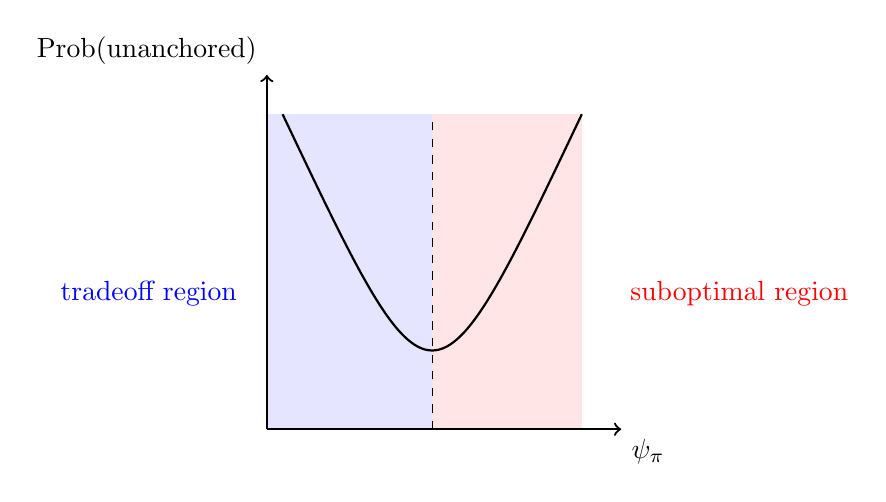
\begin{tikzpicture}
	\fill[red!10!white] (2.1,0) rectangle (4,4) ;
	 \node[below] at (6,2) {\textcolor{red}{suboptimal region}};
	 \node[below] at (-1.5,2) {\textcolor{blue}{tradeoff region}};

	\fill[blue!10!white] (0,0) rectangle (2.1,4);

\draw[thick,->] (0,0) -- (4.5,0) node[anchor=north west] {$\psi_{\pi}$};
\draw[thick,->] (0,0) -- (0,4.5) node[anchor=south east] {Prob(unanchored)};
\draw[thick] (0.2,4) .. controls (2.1,0)  .. (4,4);
\draw[dashed] (2.1,0) -- (2.1,4);
\end{tikzpicture}
\end{figure}
	\begin{lemma} \textsc{(Margin of adjustment)} \\
	Whether expectational differences between learning and rational expectations show up in inflation or the output gap depends on $\kappa$ (or equivalently $\alpha)$, the extent of nominal rigidities. A lower $\kappa$ (higher $\alpha$) means higher price rigidity and translates to output gaps being the margin of adjustment. 
	\end{lemma}
	
	\begin{conjecture} \textsc{(Optimal monetary policy)} \\
	Monetary policy under learning with endogenous gain faces two novel tradeoffs. The first is the tradeoff between overshooting and the persistence of impulse responses. On the one hand, monetary policy wishes to anchor expectations to mitigate overshooting. On the other hand, having unanchored expectations has the advantage that agents ``learn away" the shock faster. However, unanchoring leads to more volatile observables since expectations are more volatile, feeding back into endogenous variables. Thus optimal monetary policy needs to consider a) the type of shock and its severity, b) the extent of overshooting c) the desirability of getting out of the shock quickly d) and whether expectations are currently anchored, as well as how costly it would be to keep them or get them anchored. 
	
	The second tradeoff is the cost versus benefit of anchoring expectations. Having anchored expectations has the benefit of lower overshooting and volatility of observables. The cost is higher volatility of observables coming from a higher $\psi_{\pi}$ (assuming that we're in the downward-sloping part of the U-curve). Thus, ideally, monetary policy wants to ``inherit'' anchored expectations in order not to pay the cost today but enjoy the benefits.

	\end{conjecture}


\section{IRFs conditional on being anchored / unanchored}

\subsection{IRFs when changing $\rho$, anchored/unanchored}
\vspace{-0.5cm}
\begin{figure}[h!]
\subfigure[\colorbox{yellow}{$\rho$ = 0}]{\includegraphics[scale = \mySmallerFigScale]{\myFigPath materials6_IRFs_intrate_smoothing_cond_anch_SORTED_natrate_rho0_psi_pi_1_5}} 
\subfigure[\colorbox{yellow}{$\rho$ = 0.3}]{\includegraphics[scale = \mySmallerFigScale]{\myFigPath materials6_IRFs_intrate_smoothing_cond_anch_SORTED_natrate_rho0_3_psi_pi_1_5} }
\subfigure[\colorbox{yellow}{$\rho$ = 0.6}]{\includegraphics[scale = \mySmallerFigScale]{\myFigPath materials6_IRFs_intrate_smoothing_cond_anch_SORTED_natrate_rho0_6_psi_pi_1_5} }
\subfigure[\colorbox{yellow}{$\rho$ = 0.9}]{\includegraphics[scale = \mySmallerFigScale]{\myFigPath materials6_IRFs_intrate_smoothing_cond_anch_SORTED_natrate_rho0_9_psi_pi_1_5} }
\caption{IRFs to a natural rate shock ($r^n$)}
\end{figure}

\vspace{-0.5cm}
\begin{figure}[h!]
\subfigure[\colorbox{yellow}{$\rho$ = 0}]{\includegraphics[scale = \mySmallerFigScale]{\myFigPath materials6_IRFs_intrate_smoothing_cond_anch_SORTED_monpol_rho0_psi_pi_1_5}} 
\subfigure[\colorbox{yellow}{$\rho$ = 0.3}]{\includegraphics[scale = \mySmallerFigScale]{\myFigPath materials6_IRFs_intrate_smoothing_cond_anch_SORTED_monpol_rho0_3_psi_pi_1_5} }
\subfigure[\colorbox{yellow}{$\rho$ = 0.6}]{\includegraphics[scale = \mySmallerFigScale]{\myFigPath materials6_IRFs_intrate_smoothing_cond_anch_SORTED_monpol_rho0_6_psi_pi_1_5} }
\subfigure[\colorbox{yellow}{$\rho$ = 0.9}]{\includegraphics[scale = \mySmallerFigScale]{\myFigPath materials6_IRFs_intrate_smoothing_cond_anch_SORTED_monpol_rho0_9_psi_pi_1_5} }
\caption{IRFs to a monetary policy shock ($\bar{i}$)}
\end{figure}
\vspace{-0.5cm}
\begin{figure}[h!]
\subfigure[\colorbox{yellow}{$\rho$ = 0}]{\includegraphics[scale = \mySmallerFigScale]{\myFigPath materials6_IRFs_intrate_smoothing_cond_anch_SORTED_costpush_rho0_psi_pi_1_5}} 
\subfigure[\colorbox{yellow}{$\rho$ = 0.3}]{\includegraphics[scale = \mySmallerFigScale]{\myFigPath materials6_IRFs_intrate_smoothing_cond_anch_SORTED_costpush_rho0_3_psi_pi_1_5} }
\subfigure[\colorbox{yellow}{$\rho$ = 0.6}]{\includegraphics[scale = \mySmallerFigScale]{\myFigPath materials6_IRFs_intrate_smoothing_cond_anch_SORTED_costpush_rho0_6_psi_pi_1_5} }
\subfigure[\colorbox{yellow}{$\rho$ = 0.9}]{\includegraphics[scale = \mySmallerFigScale]{\myFigPath materials6_IRFs_intrate_smoothing_cond_anch_SORTED_costpush_rho0_9_psi_pi_1_5} }
\caption{IRFs to a cost-push shock ($u$)}
\end{figure}

\clearpage	
\subsection{Gain conditional on shocks when changing $\rho$, anchored/unanchored}
\begin{figure}[h!]
\subfigure[\colorbox{yellow}{$\rho$ = 0}]{\includegraphics[scale = \myTinierFigScale]{\myFigPath materials6_cond_anch_gain_natrate_rho0_psi_pi_1_5}} 
\subfigure[\colorbox{yellow}{$\rho$ = 0.3}]{\includegraphics[scale = \myTinierFigScale]{\myFigPath materials6_cond_anch_gain_natrate_rho0_3_psi_pi_1_5} }
\subfigure[\colorbox{yellow}{$\rho$ = 0.6}]{\includegraphics[scale = \myTinierFigScale]{\myFigPath materials6_cond_anch_gain_natrate_rho0_6_psi_pi_1_5} }
\subfigure[\colorbox{yellow}{$\rho$ = 0.9}]{\includegraphics[scale = \myTinierFigScale]{\myFigPath materials6_cond_anch_gain_natrate_rho0_9_psi_pi_1_5} }
\caption{Mean gain and drift after a natural rate shock ($r^n$)}
\end{figure}
\begin{figure}[h!]
\subfigure[\colorbox{yellow}{$\rho$ = 0}]{\includegraphics[scale = \myTinierFigScale]{\myFigPath materials6_cond_anch_gain_monpol_rho0_psi_pi_1_5}} 
\subfigure[\colorbox{yellow}{$\rho$ = 0.3}]{\includegraphics[scale = \myTinierFigScale]{\myFigPath materials6_cond_anch_gain_monpol_rho0_3_psi_pi_1_5} }
\subfigure[\colorbox{yellow}{$\rho$ = 0.6}]{\includegraphics[scale = \myTinierFigScale]{\myFigPath materials6_cond_anch_gain_monpol_rho0_6_psi_pi_1_5} }
\subfigure[\colorbox{yellow}{$\rho$ = 0.9}]{\includegraphics[scale = \myTinierFigScale]{\myFigPath materials6_cond_anch_gain_monpol_rho0_9_psi_pi_1_5} }
\caption{Mean gain and drift after a monetary policy shock ($\bar{i}$)}
\end{figure}
\begin{figure}[h!]
\subfigure[\colorbox{yellow}{$\rho$ = 0}]{\includegraphics[scale = \myTinierFigScale]{\myFigPath materials6_cond_anch_gain_costpush_rho0_psi_pi_1_5}} 
\subfigure[\colorbox{yellow}{$\rho$ = 0.3}]{\includegraphics[scale = \myTinierFigScale]{\myFigPath materials6_cond_anch_gain_costpush_rho0_3_psi_pi_1_5} }
\subfigure[\colorbox{yellow}{$\rho$ = 0.6}]{\includegraphics[scale = \myTinierFigScale]{\myFigPath materials6_cond_anch_gain_costpush_rho0_6_psi_pi_1_5} }
\subfigure[\colorbox{yellow}{$\rho$ = 0.9}]{\includegraphics[scale = \myTinierFigScale]{\myFigPath materials6_cond_anch_gain_costpush_rho0_9_psi_pi_1_5} }
\caption{Mean gain and drift after a cost-push shock ($u$)}
\end{figure}

\clearpage
\subsection{IRFs when changing $\psi_{\pi} (\rho =0)$, anchored/unanchored}
\begin{figure}[h!]
\subfigure[\colorbox{yellow}{$\psi_{\pi} $ = 1.1}]{\includegraphics[scale = \mySmallerFigScale]{\myFigPath materials6_IRFs_intrate_smoothing_cond_anch_SORTED_natrate_rho0_psi_pi_1_1}} 
\subfigure[\colorbox{yellow}{$\psi_{\pi} $ = 1.5}]{\includegraphics[scale = \mySmallerFigScale]{\myFigPath materials6_IRFs_intrate_smoothing_cond_anch_SORTED_natrate_rho0_psi_pi_1_5} }
\subfigure[\colorbox{yellow}{$\psi_{\pi} $ = 2}]{\includegraphics[scale = \mySmallerFigScale]{\myFigPath materials6_IRFs_intrate_smoothing_cond_anch_SORTED_natrate_rho0_psi_pi_2} }
\caption{IRFs to a natural rate shock ($r^n$)}
\end{figure}

\begin{figure}[h!]
\subfigure[\colorbox{yellow}{$\psi_{\pi} $ = 1.1}]{\includegraphics[scale = \mySmallerFigScale]{\myFigPath materials6_IRFs_intrate_smoothing_cond_anch_SORTED_monpol_rho0_psi_pi_1_1}} 
\subfigure[\colorbox{yellow}{$\psi_{\pi} $ = 1.5}]{\includegraphics[scale = \mySmallerFigScale]{\myFigPath materials6_IRFs_intrate_smoothing_cond_anch_SORTED_monpol_rho0_psi_pi_1_5} }
\subfigure[\colorbox{yellow}{$\psi_{\pi} $ = 2}]{\includegraphics[scale = \mySmallerFigScale]{\myFigPath materials6_IRFs_intrate_smoothing_cond_anch_SORTED_monpol_rho0_psi_pi_2} }
\caption{IRFs to a monetary policy shock ($\bar{i}$)}
\end{figure}

\begin{figure}[h!]
\subfigure[\colorbox{yellow}{$\psi_{\pi} $ = 1.1}]{\includegraphics[scale = \mySmallerFigScale]{\myFigPath materials6_IRFs_intrate_smoothing_cond_anch_SORTED_costpush_rho0_psi_pi_1_1}} 
\subfigure[\colorbox{yellow}{$\psi_{\pi} $ = 1.5}]{\includegraphics[scale = \mySmallerFigScale]{\myFigPath materials6_IRFs_intrate_smoothing_cond_anch_SORTED_costpush_rho0_psi_pi_1_5} }
\subfigure[\colorbox{yellow}{$\psi_{\pi} $ = 2}]{\includegraphics[scale = \mySmallerFigScale]{\myFigPath materials6_IRFs_intrate_smoothing_cond_anch_SORTED_costpush_rho0_psi_pi_2} }
\caption{IRFs to a cost-push shock ($u$)}
\end{figure}

\clearpage
\subsection{Gain conditional on shocks when changing $\psi_{\pi}$,  anchored/unanchored}
\begin{figure}[h!]
\subfigure[\colorbox{yellow}{$\psi_{\pi} $ = 1.1}]{\includegraphics[scale = \myTinierFigScale]{\myFigPath materials6_cond_anch_gain_natrate_rho0_psi_pi_1_1}} 
\subfigure[\colorbox{yellow}{$\psi_{\pi} $ = 1.5}]{\includegraphics[scale = \myTinierFigScale]{\myFigPath materials6_cond_anch_gain_natrate_rho0_psi_pi_1_5} }
\subfigure[\colorbox{yellow}{$\psi_{\pi} $ = 2}]{\includegraphics[scale = \myTinierFigScale]{\myFigPath materials6_cond_anch_gain_natrate_rho0_psi_pi_2} }
\caption{Mean gain and drift after a natural rate shock ($r^n$)}
\end{figure}
\begin{figure}[h!]
\subfigure[\colorbox{yellow}{$\psi_{\pi} $ = 1.1}]{\includegraphics[scale = \myTinierFigScale]{\myFigPath materials6_cond_anch_gain_monpol_rho0_psi_pi_1_1}} 
\subfigure[\colorbox{yellow}{$\psi_{\pi} $ = 1.5}]{\includegraphics[scale = \myTinierFigScale]{\myFigPath materials6_cond_anch_gain_monpol_rho0_psi_pi_1_5} }
\subfigure[\colorbox{yellow}{$\psi_{\pi} $ = 2}]{\includegraphics[scale = \myTinierFigScale]{\myFigPath materials6_cond_anch_gain_monpol_rho0_psi_pi_2} }
\caption{Mean gain and drift after a monetary policy shock ($\bar{i}$)}
\end{figure}
\begin{figure}[h!]
\subfigure[\colorbox{yellow}{$\psi_{\pi} $ = 1.1}]{\includegraphics[scale = \myTinierFigScale]{\myFigPath materials6_cond_anch_gain_costpush_rho0_psi_pi_1_1}} 
\subfigure[\colorbox{yellow}{$\psi_{\pi} $ = 1.5}]{\includegraphics[scale = \myTinierFigScale]{\myFigPath materials6_cond_anch_gain_costpush_rho0_psi_pi_1_5} }
\subfigure[\colorbox{yellow}{$\psi_{\pi} $ = 2}]{\includegraphics[scale = \myTinierFigScale]{\myFigPath materials6_cond_anch_gain_costpush_rho0_psi_pi_2} }
\caption{Mean gain and drift after a cost-push shock ($u$)}
\end{figure}






\end{document}





